%!TEX root = ../main.tex

\section{Annexe}
\label{sec:annexe}


\begin{figure}
  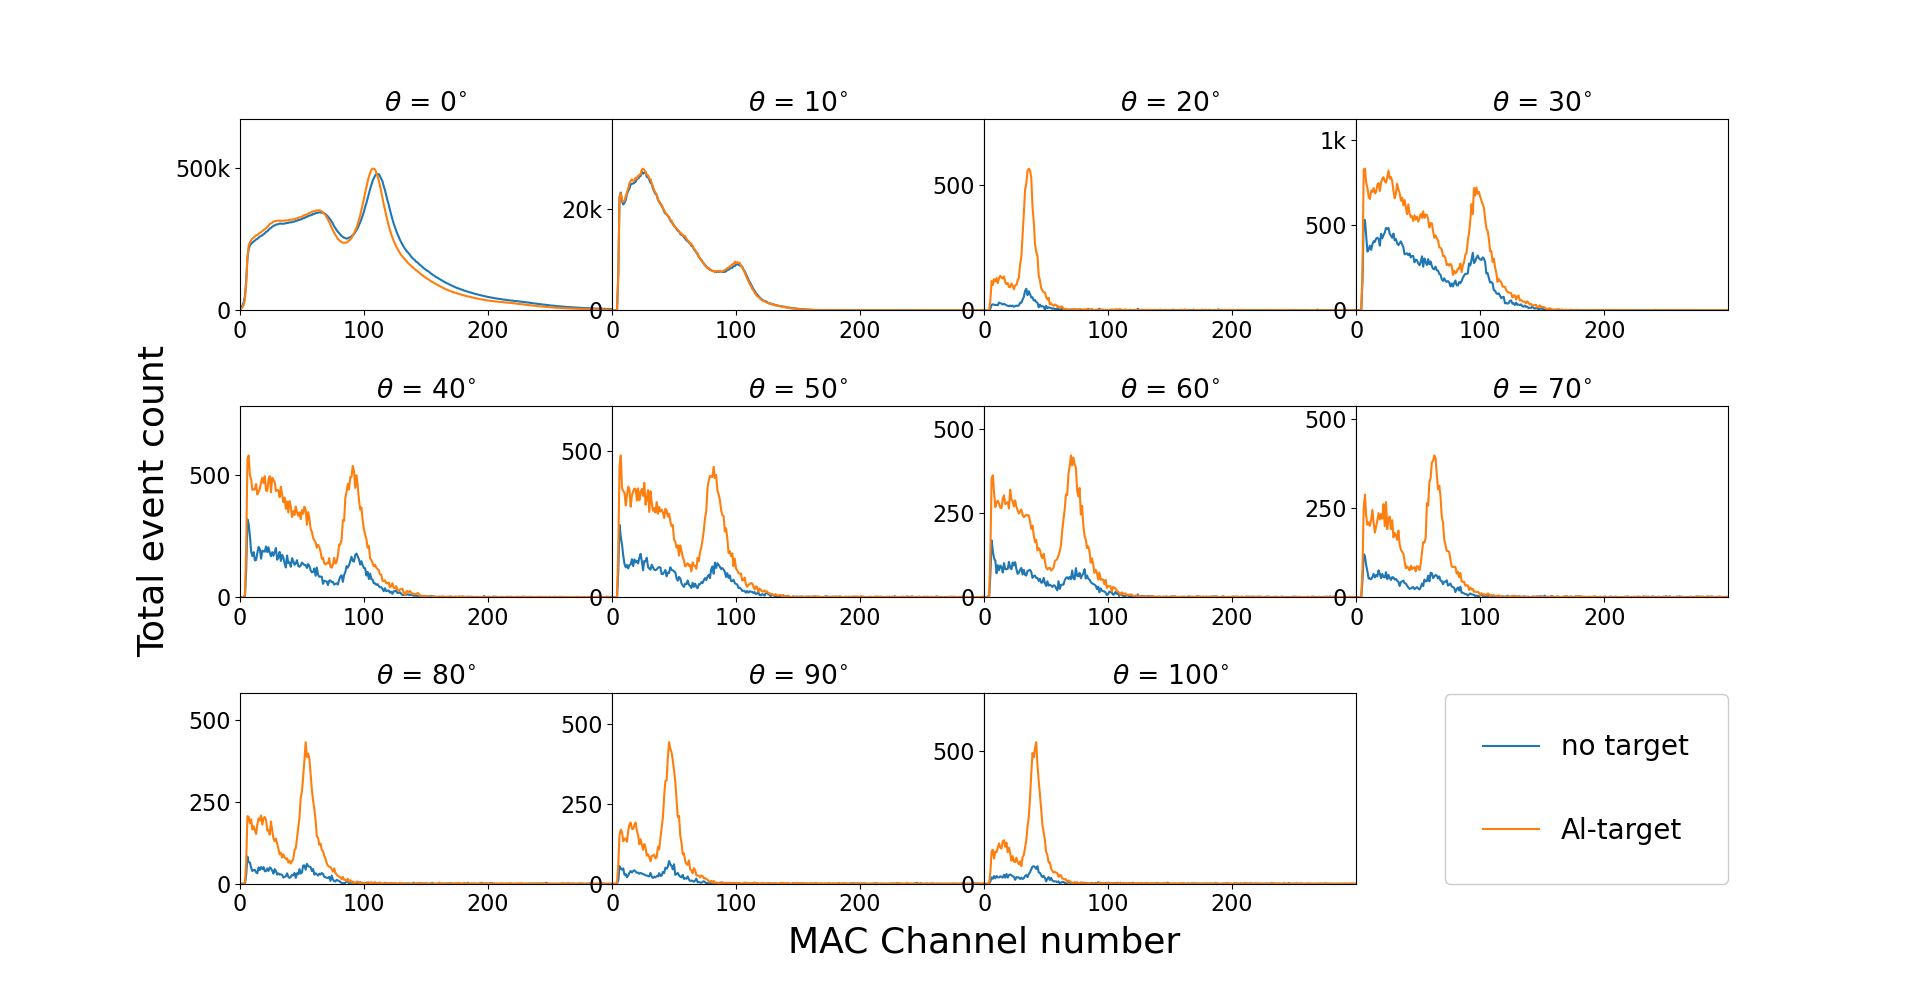
\includegraphics[width=1.0\textwidth]{./fig/differential measurements.png}
\caption{Raw number of events counted in every channel for each measured angle.
  The dashed black lines indicate the theoretical energy a photon has after
  undergoing compton scattering at an angle $\theta$. The distance between signal
  peaks and this energy grows with increasing scattering angles. This is expected
  due to the imperfect calibration.}\label{fig:diff-measurements2}
\end{figure}

\begin{figure}
  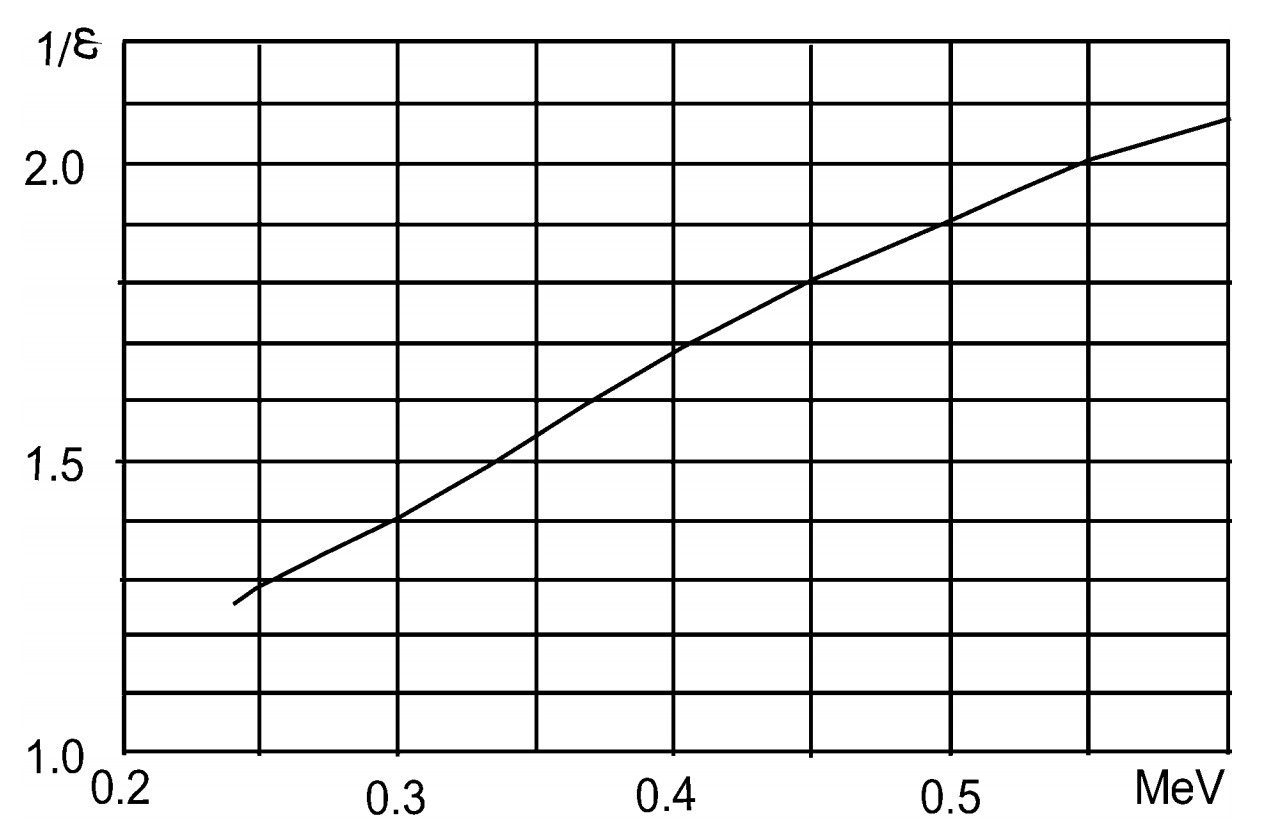
\includegraphics[width=1.0\textwidth]{./fig/plot710.png}
\caption{Sensitivity correction for the NaJ crystal from Plot 7.10 (p.134) in \cite{Sch17}.}\label{fig:plot710}
\end{figure}